\documentclass{utue} %uumi.cls required for Uni corporate design
\usepackage{listings}
\usepackage{url}

\lstset{numbers=left, numberstyle=\tiny, numbersep=5pt, xleftmargin=10mm}

% Values for title generation
\title{Funfair: game control with EEG}
\author{Robert Eisele \& Robert Geirhos}
\date{\today}

% Subtitle is optional. It represents what kind of work you did.
\subtitle{Praktikum Computergrafik WS2016/17}

\begin{document}

% You can place a teaser as follows. (Otherwise, just uncomment the following part)
\teaser{
    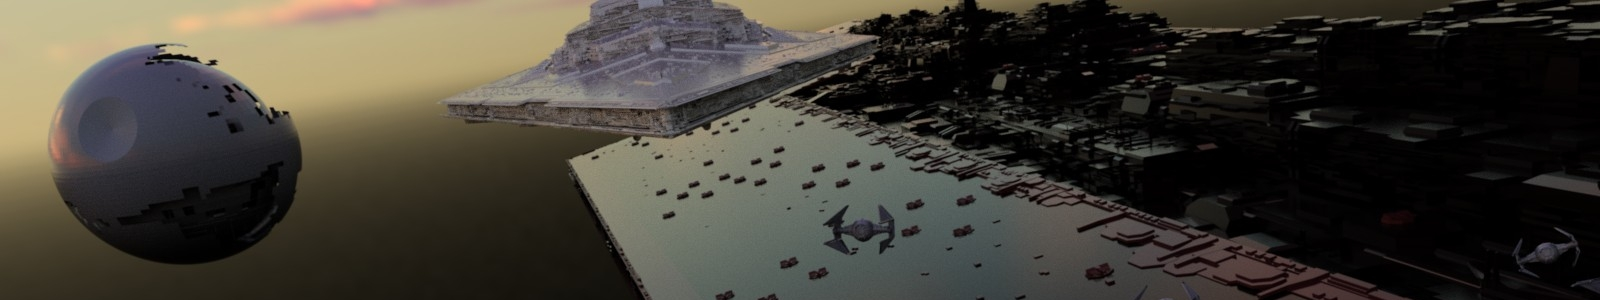
\includegraphics[width=\textwidth]{images/teaser.jpg}
    \caption{You can place a teaser here.}
    \label{fig:teaser}
}     

% Creates title of document and additional title page.
\maketitle

\section*{Abstract}

Electroencephalography (EEG) is a technique for measuring brain activity. Although widely used in neuroscientific research, it has thus far only rarely been used for the purpose of computer game control. Here we show that a leightweight EEG device, the Emotiv XXX, can be successfully used to play a broad range of simple yet challenging computer games. Furthermore, we demonstrate that rather than merely substituting a mouse or keyboard, an EEG device enables the development of a new type of games which go beyond traditional means of game control. We specifically developed six games, all of which can be played by controlling one's mental activity. We anticipate our work to be a starting point for ever more complex games and a new, keyboard-free gaming experience.


% Give an overview over your project here. Give a glimpse insight in the problem and write why it is important to be solved. Write what you did to make your implementation better than the state of the art implementations.


\section{Introduction}

Give an introduction to the problem. This might start from history, motivate the problem and end with the computational demands. Motivate why to use GPUs. You should also introduce CUDA in a way that makes an average computer science student understand what it is.


\section{Description of the Solution}

Describe your solution to the problem in detail. I propose to spend one chapter on a general, simple solution strategy so that the reader is familiar with how to solve the problem. This could also be a summary of the paper or document you mainly used to base your work on.

Subsequently, your particular solution should be described. Spend at least one chapter on describing the (parallel) improvements you made upon the naive implementation. It might be advantageous to split the implementation description to parts, each filling a subsection, and to give an overview over those parts first.

\subsection{Subsection}

Subsections look like this. If you need more hierarchy, use paragraphs.

\section{Possible Extensions}

Describe possible extensions and discuss why they could be useful.


\appendix

\section{General Infos}

You don't need an appendix. The two appendix sections are just there to give some additional or general information.

This document describes roughly, what the documentation of the Praktikum project should look like.

Note that your final documentation of your project should contain 6 text pages using this template plus the cover and the empty sheet at the beginning. Within the 6 pages, at least 4 pages should be only text.

\section{\LaTeX~Infos}

This section demonstrates some \LaTeX~features / characteristics. For a much more extensive introduction to \LaTeX, refer to the PDF on \url{http://drzoom.ch/diplomarbeit-mit-latex.html}. For getting certain LaTeX features and keywords explained, have a look at \url{http://en.wikibooks.org/wiki/LaTeX}

\begin{figure}[h!]
  \centering
  
\includegraphics[width=.4\columnwidth]{images/Tuebingen_CorporateElements/UT_BM_Rot_RGB_tr_01.png}
  \caption{This is a figure.}
  \label{fig:figure1}
\end{figure}

You should refere to images like the one in Figure \ref{fig:figure1} from the text instead of trying to place figures close to the text parts where they are mentioned. You cannot force \LaTeX~to place images on certain positions but only give it some hints, so make sure that your document is understandable independently from figure placement.

Beside figures, you can also label sections and tables and refer to them.

For references, extend the \texttt{bibliography.bib} file and cite papers like \cite{Miller1995}. The easiest way to edit the \texttt{.bib} file is to use a tool like \emph{Jabref}. You may also find ready to use bibtex tags on the web which you can directly copy to the \texttt{bibliography.bib} file.

For building this document, you should use 
\begin{lstlisting}[firstnumber=1]
pdflatex reportTemplate.tex
bibtex reportTemplate.aux
pdflatex reportTemplate.tex
pdflatex reportTemplate.tex
\end{lstlisting}
to be sure that all citations and references within the document are correct. In some weired cases, it might be necessary to run pdflatex even more often.

Remember to change your \LaTeX~source in small steps - this makes error tracking quite easy.


\bibliographystyle{alpha}
\bibliography{bibliography}

\end{document}

